\documentclass{beamer}
\usepackage[utf8]{inputenc}

\usetheme{Madrid}
\usecolortheme{default}
\usepackage{amsmath,amssymb,amsfonts,amsthm}
\usepackage{txfonts}
\usepackage{tkz-euclide}
\usepackage{listings}
\usepackage{adjustbox}
\usepackage{array}
\usepackage{tabularx}
\usepackage{gvv}
\usepackage{lmodern}
\usepackage{circuitikz}
\usepackage{tikz}
\usepackage{graphicx}

\setbeamertemplate{page number in head/foot}[totalframenumber]

\usepackage{tcolorbox}
\tcbuselibrary{minted,breakable,xparse,skins}



\definecolor{bg}{gray}{0.95}
\DeclareTCBListing{mintedbox}{O{}m!O{}}{%
  breakable=true,
  listing engine=minted,
  listing only,
  minted language=#2,
  minted style=default,
  minted options={%
    linenos,
    gobble=0,
    breaklines=true,
    breakafter=,,
    fontsize=\small,
    numbersep=8pt,
    #1},
  boxsep=0pt,
  left skip=0pt,
  right skip=0pt,
  left=25pt,
  right=0pt,
  top=3pt,
  bottom=3pt,
  arc=5pt,
  leftrule=0pt,
  rightrule=0pt,
  bottomrule=2pt,
  toprule=2pt,
  colback=bg,
  colframe=orange!70,
  enhanced,
  overlay={%
    \begin{tcbclipinterior}
    \fill[orange!20!white] (frame.south west) rectangle ([xshift=20pt]frame.north west);
    \end{tcbclipinterior}},
  #3,
}
\lstset{
    language=C,
    basicstyle=\ttfamily\small,
    keywordstyle=\color{blue},
    stringstyle=\color{orange},
    commentstyle=\color{green!60!black},
    numbers=left,
    numberstyle=\tiny\color{gray},
    breaklines=true,
    showstringspaces=false,
}
\begin{document}

\title 
{5.8.31}
\date{September 13,2025}


\author 
{Kavin B-EE25BTECH11033}






\frame{\titlepage}
\begin{frame}{Question}
In a $\triangle ABC,  \angle C=3 \angle B=2(\angle A+\angle B)$.  Find the three angles. 
\bigskip
\end{frame}



\begin{frame}{Theoretical Solution}
In a $\triangle ABC$ , the sum of interior angles is equal to $180$.
\begin{align}
    \angle A + \angle B + \angle C = 180
\end{align}
Also,
\begin{align}
    \angle C - 3\angle B = 0
\end{align}
\begin{align}
    2\angle A - \angle B = 0
\end{align}
\end{frame}

\begin{frame}{Theoretical Solution}
On putting the above equations in a matrix we will get,
\begin{align}
    \myvec{ 1 & 1 & 1\\0 & -3 & 1\\2 & -1 & 0}\myvec{\angle A \\ \angle B \\ \angle C} = \myvec{180\\0\\0}
\end{align}
The augmented matrix is given by,
\begin{align}
    \augvec{3}{1}{1 & 1 & 1 & 180\\0 & -3 & 1 & 0\\2 & -1 & 0 & 0}
\end{align}
\end{frame}


\begin{frame}{Theoretical Solution}
\begin{align}
    R_3 \to R_3 - 2R_1 \implies \augvec{3}{1}{1 & 1 & 1 & 180 \\ 0 & -3 & 1 & 0 \\ 0 & -3 & -2 & -360}
\end{align}
\begin{align}
    R_2 \to -1/3 R_2  \implies \augvec{3}{1}{1 & 1 & 1 & 180 \\ 0 & 1 & -1/3 & 0 \\ 0 & -3 & -2 & -360}
\end{align}
\begin{align}
    R_1 \to R_1 - R_2\ \text{and}\ R_3 \to R_3 + 3R_2 \implies \augvec{3}{1}{1 & 0 & 4/3 & 180 \\ 0 & 1 & -1/3 & 0 \\ 0 & 0 & -3 & -360}
\end{align}
\end{frame}
\begin{frame}{Theoretical Solution}
\begin{align}
    R_3 \to -1/3 R_3 \implies \augvec{3}{1}{1 & 0 & 4/3 & 180 \\ 0 & 1 & -1/3 & 0 \\ 0 & 0 & 1 & 120}
\end{align}
\begin{align}
    R_1 \to R_1 - 4/3 R_3\ \text{and}\ R_2 \to R_2 + 1/3 R_3\implies \augvec{3}{1}{1 & 0 & 0 & 20 \\ 0 & 1 & 0 & 40 \\ 0 & 0 & 1 & 120}
\end{align}
\begin{align}
    \implies \myvec{\angle A \\ \angle B \\ \angle C} = \myvec{20\\40\\120}
\end{align}
Therefore,
\begin{align*}
\angle A = 20\degree \ \ \ \ \ 
\angle B = 40\degree
\end{align*}
\begin{align*}
\angle C = 120\degree
\end{align*}
\end{frame}

\begin{frame}{Plot}
    \centering
    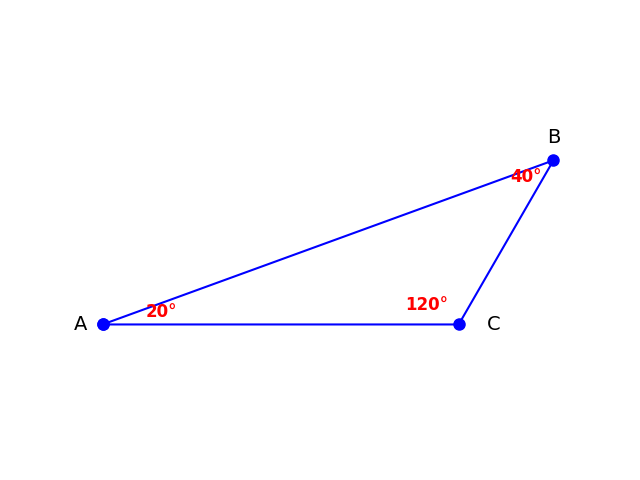
\includegraphics[width=\columnwidth, height=0.8\textheight, keepaspectratio]{figs/fig.png}
\end{frame}


\end{document}
